\bookchapter{The GameController protocol}\label{ch:rc3}

\section*{Explanation}
How does a robot know that the referee has whistled, that it has been penalised, or that its team has $11\,650$ messages left? From the \textbf{GameController}, a program on a laptop at the side of the field that is operated by a person (the GameController operator) and talks to all robots over the network. The official GameController of the HSL is written in \textbf{Rust}: a Cargo workspace with a graphical interface in \texttt{egui}, a core library with the game logic, a crate for the messages, a crate for the network (\texttt{tokio}), an automatic referee for simulators, a C interface and Python bindings, and a tool that analyses the log files. Everything you learned in Part~\ref{part:rust} is in it.

\begin{keyidea}[There are many GameControllers; use the official one]
Over the years many versions of the GameController have existed (for the SPL, for the older humanoid leagues, forks). The one that is used in the HSL today is the repository \texttt{RoboCup-HumanoidSoccerLeague/GameController}. Its documentation says that its network protocol is defined by one C header, \verb!RoboCupGameControlData.h!. When you read an older tutorial about another GameController, check the \emph{version number} in the header (this chapter: control packets version $20$, return packets version $4$).
\end{keyidea}

\section*{Three channels}
The communication consists of three UDP channels. (UDP and sockets: Chapter~\ref{ch:rust7}.)

\begin{center}
\begin{tikzpicture}[>={Stealth[length=2.2mm]},bx/.style={draw,thick,rounded corners=3pt,minimum height=0.9cm,font=\small,align=center}]
 \node[bx,fill=orange!15,minimum width=3cm] (gc) at (0,0) {GameController\\ (operator laptop)};
 \node[bx,fill=gray!15,minimum width=2.2cm] (ap) at (5,0) {access point};
 \node[bx,fill=blue!10,minimum width=2.2cm] (r1) at (9,1.3) {robot 1};
 \node[bx,fill=blue!10,minimum width=2.2cm] (r2) at (9,0) {robot 2};
 \node[bx,fill=blue!10,minimum width=2.2cm] (r3) at (9,-1.3) {robot $n$};
 \draw[->,thick] (gc.north east) to[out=40,in=140] node[above,font=\scriptsize,align=center]{control, broadcast, port 3838\\ 2\,Hz} (ap.north west);
 \draw[->,thick,red!70!black] (ap.south west) to[out=-140,in=-40] node[below,font=\scriptsize,align=center]{status, unicast, port 3939\\ 0.5--2\,Hz} (gc.south east);
 \foreach \r in {r1,r2,r3}{\draw[thick] (ap)--(\r);}
 \draw[<->,thick,green!40!black] (r1.east) to[out=0,in=0,looseness=1.6] node[right,font=\scriptsize,align=center]{team messages\\ broadcast, port\\ $10000+$ team no.} (r3.east);
\end{tikzpicture}
\captionof{figure}{The three channels. The GameController broadcasts the game state; every robot answers with a short status packet; and the robots of a team talk to each other on a port that is $10000$ plus the team number. All traffic goes through the access point of the field; direct ad-hoc connections between robots are forbidden.}
\end{center}

\begin{description}[leftmargin=0.6cm]
 \item[Control message] The GameController sends the \emph{game state} as a UDP \textbf{broadcast} to port $3838$, twice per second. It does not always show the true state: after a transition to \emph{playing} the old state is kept for up to $10$\,s (the delay of Chapter~\ref{ch:rc2}). When play is stopped, a packet is sent at once and the rate rises to $5$\,Hz.
 \item[Status message] Each robot has to send a \textbf{return packet} to the GameController (unicast, port $3939$) at a rate between $0.5$ and $2$\,Hz. It says who the robot is, whether it has fallen, where it believes to be, and where it sees the ball.
 \item[Team messages] The robots of a team broadcast messages with free format (at most $512$ bytes of payload) to the port $10000+$ team number. The GameController \emph{listens} to this port only to \textbf{count} the messages and their size (Chapter~\ref{ch:rc4}).
\end{description}
There is a fourth interface for \textbf{monitors} (programs that show the true game state, for example for the audience): they register on port $3636$ with the four bytes \texttt{RGTr} and a version byte and receive the true control messages. A host that has sent status messages is refused, because it is assumed to be a robot that must not receive the true data.

\section*{The control message: $158$ bytes}
The message is a C struct with fixed size, written byte by byte on the network (all numbers little-endian, as on the usual processors). The figure shows its layout; the numbers are the offsets that the C compiler produces for the header of the GameController (this was checked: a small C program with the real header prints \verb!sizeof! $=158$, the offset of the first team $18$, and the size of one team $70$).

\begin{center}
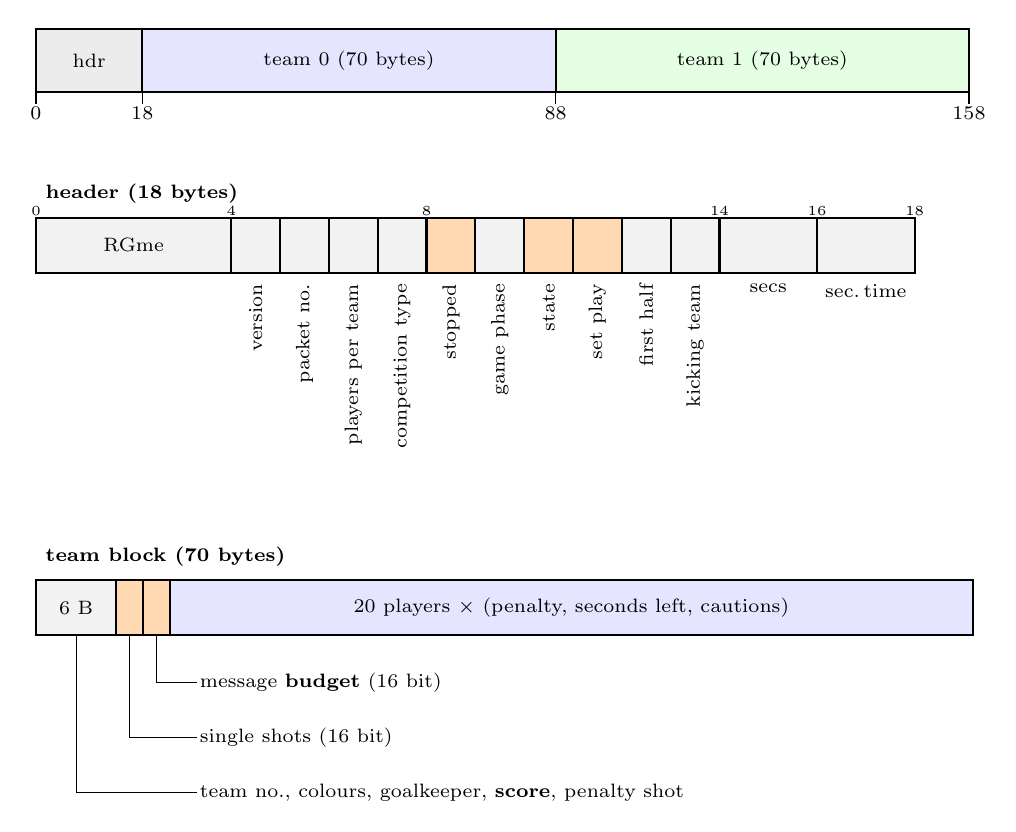
\begin{tikzpicture}[font=\scriptsize]
 % overview bar (0.075 cm per byte)
 \begin{scope}[x=0.075cm,y=1cm]
  \draw[thick,fill=gray!15] (0,0) rectangle (18,0.8);
  \draw[thick,fill=blue!10] (18,0) rectangle (88,0.8);
  \draw[thick,fill=green!10] (88,0) rectangle (158,0.8);
  \node at (9,0.4) {hdr}; \node at (53,0.4) {team 0 (70 bytes)}; \node at (123,0.4) {team 1 (70 bytes)};
  \foreach \x in {0,18,88,158}{\draw (\x,0)--(\x,-0.15); \node[below,inner sep=1pt] at (\x,-0.15) {\x};}
 \end{scope}
 % zoom of the header: 0.62 cm per byte
 \begin{scope}[shift={(0,-2.3)},x=0.62cm,y=1cm]
  \node[anchor=west,font=\scriptsize\bfseries] at (0,1.0) {header (18 bytes)};
  \foreach \a/\b/\t/\f in {0/4/RGme/gray!10,4/5/version/gray!10,5/6/packet no./gray!10,6/7/players per team/gray!10,7/8/competition/gray!10,8/9/stopped/orange!30,9/10/game phase/gray!10,10/11/state/orange!30,11/12/set play/orange!30,12/13/first half/gray!10,13/14/kicking team/gray!10,14/16/secs remaining/gray!10,16/18/secondary time/gray!10}{
   \draw[thick,fill=\f] (\a,0) rectangle (\b,0.7);
  }
  \node at (2,0.35) {RGme};
  \foreach \a/\t in {4/version,5/packet no.,6/players per team,7/competition type,8/stopped,9/game phase,10/state,11/set play,12/first half,13/kicking team}{
   \node[rotate=90,anchor=east,inner sep=1pt] at (\a+0.5,-0.1) {\t};
  }
  \node[anchor=north,inner sep=1pt] at (15,-0.1) {secs};
  \node[anchor=north,inner sep=1pt] at (17,-0.1) {sec.\,time};
  \foreach \a in {0,4,8,14,16,18}{\node[above,font=\tiny,inner sep=0.5pt] at (\a,0.7) {\a};}
 \end{scope}
 % zoom of a team block: 0.17 cm per byte
 \begin{scope}[shift={(0,-6.9)},x=0.17cm,y=1cm]
  \node[anchor=west,font=\scriptsize\bfseries] at (0,1.0) {team block (70 bytes)};
  \draw[thick,fill=gray!10] (0,0) rectangle (6,0.7);
  \draw[thick,fill=orange!30] (6,0) rectangle (8,0.7);
  \draw[thick,fill=orange!30] (8,0) rectangle (10,0.7);
  \draw[thick,fill=blue!10] (10,0) rectangle (70,0.7);
  \node at (3,0.35) {6 B}; \node at (40,0.35) {20 players $\times$ (penalty, seconds left, cautions)};
  \draw (9,0)--(9,-0.6)--(12,-0.6); \node[anchor=west,inner sep=1pt] at (12,-0.6) {message \textbf{budget} (16 bit)};
  \draw (7,0)--(7,-1.3)--(12,-1.3); \node[anchor=west,inner sep=1pt] at (12,-1.3) {single shots (16 bit)};
  \draw (3,0)--(3,-2.0)--(12,-2.0); \node[anchor=west,inner sep=1pt] at (12,-2.0) {team no., colours, goalkeeper, \textbf{score}, penalty shot};
 \end{scope}
\end{tikzpicture}
\captionof{figure}{The $158$ bytes of the control message. The sizes of the header, $18$, and of a team, $70$, follow from the field sizes; no padding is needed, because the $16$-bit fields fall on even offsets.}
\end{center}

The fields that your behaviour needs most are a handful: the \textbf{state} (initial, ready, set, playing, finished), \textbf{stopped}, the \textbf{set play} and \textbf{kicking team} (who has the free kick), the \textbf{seconds remaining} and \textbf{secondary time} (what is shown as the second clock, for example the rest of \emph{ready}), the \textbf{score}, the \textbf{message budget} and, per player, the \textbf{penalty} and the seconds until it ends. Colours are only needed to check that your jersey matches.

\section*{The return message: $32$ bytes}
\begin{center}
\small
\begin{tabular}{rlll}
\hline
offset & field & type & meaning\\
\hline
0 & header \texttt{RGrt} & 4 bytes & \\
4 & version & byte & $4$\\
5, 6 & player number, team number & bytes & player number starts at $1$\\
7 & fallen & byte & $1$ if the robot lies\\
8, 12, 16 & pose $x,y,\theta$ & 3 floats & mm, mm, rad; $x$ towards the opponent's goal\\
20 & ball age & float & seconds since the ball was seen, $-1$ if never\\
24, 28 & ball $x,y$ & 2 floats & millimetres relative to the robot\\
\hline
\end{tabular}
\end{center}
This packet is the \textbf{only way} in which the referee software knows where your robots are. It is a good test of your localisation (Chapter~\ref{ch:ctl5}): the log files of the GameController contain your poses, and you can compare them with the video.

\section*{A parser in Rust}
The program below reads the control message, checks it as the GameController does (length, header and version), and builds the return message. It uses only the standard library. It was compiled and tested against a message produced by a C program with the \emph{real} header file of the GameController: all fields come out right, the return packet is identical byte for byte to the C struct, and a packet that is too short or has an old version is rejected.

\begin{verbatim}
const HEADER: &[u8; 4] = b"RGme";
const VERSION: u8 = 20;
pub const CONTROL_LEN: usize = 158;

#[derive(Debug, Clone, Copy, PartialEq)]
pub enum State { Initial, Ready, Set, Playing, Finished }

#[derive(Debug, Clone, Copy, Default)]
pub struct Player { pub penalty: u8, pub secs_left: u8, pub cautions: u8 }

#[derive(Debug, Clone)]
pub struct Team {
    pub number: u8,
    pub score: u8,
    pub goalkeeper: u8,
    pub message_budget: u16,
    pub players: [Player; 20],
}

#[derive(Debug, Clone)]
pub struct Control {
    pub packet_number: u8,
    pub stopped: bool,
    pub state: State,
    pub set_play: u8,
    pub first_half: bool,
    pub kicking_team: u8,
    pub secs_remaining: i16,
    pub secondary_time: i16,
    pub teams: [Team; 2],
}

fn parse_team(b: &[u8]) -> Team {
    // TeamInfo is 70 bytes: 6 x u8, u16 singleShots, u16 budget, 20 x 3 bytes
    let mut players = [Player::default(); 20];
    for (i, p) in players.iter_mut().enumerate() {
        let o = 10 + 3 * i;
        *p = Player { penalty: b[o], secs_left: b[o + 1],
                      cautions: b[o + 2] };
    }
    Team {
        number: b[0],
        score: b[4],
        goalkeeper: b[3],
        message_budget: u16::from_le_bytes([b[8], b[9]]),
        players,
    }
}

pub fn parse_control(buf: &[u8]) -> Result<Control, String> {
    if buf.len() != CONTROL_LEN {
        return Err(format!("length {}", buf.len()));
    }
    if &buf[0..4] != HEADER { return Err("bad header".into()); }
    if buf[4] != VERSION { return Err(format!("version {}", buf[4])); }
    let state = match buf[10] {
        0 => State::Initial, 1 => State::Ready, 2 => State::Set,
        3 => State::Playing, 4 => State::Finished,
        s => return Err(format!("unknown state {s}")),
    };
    Ok(Control {
        packet_number: buf[5],
        stopped: buf[8] == 1,
        state,
        set_play: buf[11],
        first_half: buf[12] == 1,
        kicking_team: buf[13],
        secs_remaining: i16::from_le_bytes([buf[14], buf[15]]),
        secondary_time: i16::from_le_bytes([buf[16], buf[17]]),
        teams: [parse_team(&buf[18..88]), parse_team(&buf[88..158])],
    })
}

pub fn encode_return(player: u8, team: u8, fallen: bool, pose: [f32; 3],
                     ball_age: f32, ball: [f32; 2]) -> [u8; 32] {
    let mut b = [0u8; 32];
    b[0..4].copy_from_slice(b"RGrt");
    b[4] = 4;
    b[5] = player;
    b[6] = team;
    b[7] = fallen as u8;
    let floats = [pose[0], pose[1], pose[2], ball_age, ball[0], ball[1]];
    for (i, f) in floats.iter().enumerate() {
        b[8 + 4 * i..12 + 4 * i].copy_from_slice(&f.to_le_bytes());
    }
    b
}
\end{verbatim}

Reading from the network looks like this (the test used the loopback address $127.0.0.1$; on a real field the robot binds the port $3838$ on its network interface):

\begin{verbatim}
use std::net::UdpSocket;
use std::time::Duration;
mod gc { include!("gc_lib.rs"); }
fn main()fn main() -> std::io::Result<()> {
    let rx = UdpSocket::bind("127.0.0.1:3838")?;
    rx.set_read_timeout(Some(Duration::from_secs(2)))?;
    let tx = UdpSocket::bind("127.0.0.1:0")?;
    tx.send_to(&std::fs::read("control.bin")?, "127.0.0.1:3838")?;
    let mut buf = [0u8; 1024];
    let (n, from) = rx.recv_from(&mut buf)?;
    match gc::parse_control(&buf[..n]) {
        Ok(c) => println!("{n} bytes from {}: {:?}, score {}:{}",
                          from.ip(), c.state,
                          c.teams[0].score, c.teams[1].score),
        Err(e) => println!("rejected: {e}"),
    }
    // reply to the GameController on the return port
    let ret = gc::encode_return(3, 12, false, [0.0; 3], -1.0, [0.0; 2]);
    let gcsock = UdpSocket::bind("127.0.0.1:3939")?;
    gcsock.set_read_timeout(Some(Duration::from_secs(2)))?;
    tx.send_to(&ret, "127.0.0.1:3939")?;
    let (m, _) = gcsock.recv_from(&mut buf)?;
    let head = std::str::from_utf8(&buf[..4]).unwrap();
    println!("return packet received: {m} bytes, header {head:?}");
    Ok(())
}
\end{verbatim}

\begin{center}
\small
\begin{tabular}{p{0.9\linewidth}}
\textbf{What was run and what was not.} Run: the parser and the encoder against the C struct, the loopback socket test (both directions), the error cases. Not run: the real GameController program (it needs a graphical environment, libclang and the crates), a real network with a robot, and the wireless access point.\\
\end{tabular}
\end{center}

\section*{Running the GameController yourself}
You can practise without a referee. According to the repository: install Rust (the project asks for a recent release; check \texttt{README.md}) and \texttt{libclang}, then \verb!cargo run -r! starts the launcher. In the launcher you choose the \textbf{competition} (for example mid, Advanced), the \textbf{home and away team}, the jersey colours, who kicks off, and the \textbf{network interface}. The operator then presses the buttons: penalty call first and then the robot, \emph{Stop play} (also on the space bar), timeouts, substitutions, and an undo timeline of the last actions. Configuration lives in YAML files: \texttt{teams.yaml} lists all teams, and each competition folder (for example \texttt{middle\_advanced}) has a \texttt{params.yaml} with the durations, penalty lengths and the message budget, for example $12000$ messages per team plus $600$ per additional minute. \textbf{To add your team} you need an entry in the global \texttt{teams.yaml} and in the \texttt{teams.yaml} of the competition. The option \texttt{--show-paths} prints where the program looks for its configuration. For automatic testing there are Python bindings (a module that returns the control message bytes) and an \textbf{autoreferee} for simulators.

\begin{aibox}[Testing against the real thing]
Your robot software should have a \textbf{GameController test}: a computer that runs the real program and a script that walks through the whole game (initial, ready, set, whistle, goal, penalty, stop, half time). Teams that test only with their own fake sender find the differences (a version number, the 10\,s delay, a changed penalty code) on the day of the competition.
\end{aibox}

\begin{keyidea}[Summary]
\begin{itemize}[nosep]
 \item Three UDP channels: control broadcast on $3838$, status unicast on $3939$, team messages on $10000+$ team number.
 \item The control message has $158$ bytes (header $18$ + two teams of $70$); the return message has $32$ bytes.
 \item Check length, header and version; ignore packets that fail the check.
 \item The state seen by the robots can be delayed by $10$\,s after \emph{playing}.
\end{itemize}
\end{keyidea}

\section*{Practice problems}
\begin{enumerate}[label=\textbf{\thechapter.\arabic*}]
  \item Compute the size of a team block ($6$ single bytes, two $16$-bit numbers and $20$ players with $3$ bytes) and of the control message. Why is it important that both sides agree on the \emph{padding}?
  \item At which byte offset of the control message is the state, and at which the message budget of the second team? (Use the figure and the table.)
  \item The GameController sends at $2$\,Hz. A robot reads the packets, but a packet is lost with probability $10\%$ (independent). What is the probability that the robot hears nothing for $2$ seconds, and what does that mean for a robot that must stop immediately on a \emph{stopped} message?
  \item Write the Python function of the chapter (with \verb!struct!) for the control message and print the state, the seconds remaining, the budget of team $0$ and the penalty of the third player of a message that you build yourself.
  \item The return packet must be sent at least every two seconds. Which part of your software sends it? What would you send as the pose if the robot is not localised?
  \item A packet arrives with version $19$ although you expect $20$. List three possible reasons and say what the robot should do.
  \item The ball age is $-1$ if the ball was never seen. How would you encode the ball position in that case? Why is it better to send the age than the time of the last observation?
  \item Explain why a broadcast needs no list of robot addresses, and what could go wrong with broadcasts on a congested wireless network.
  \item Make the loopback test of the chapter send $10$ control messages with the packet number $0\dots9$, drop packet $4$, and let the receiver print which packet numbers are missing (wrap-around at $256$).
  \item[\textbf{\thechapter.10}$\star$] Write a Rust function \verb!fn budget_left(c: &Control, team: u8) -> Option<u16>! that returns the message budget of the team with the given number, or \verb!None! if the team does not play. Then write a small program that receives control messages and prints a warning when the budget falls below $1000$, or when the packet number jumps by more than one (a lost packet).
\end{enumerate}
